\chapter{Задание для тренировки}

\textbf{Вариант}: 1

\textbf{Задание}: Осуществить планирование проекта со следующими временными характеристиками.

\begin{table}[!h]
	\begin{center}
		\caption{Временные характеристики проекта}
		\begin{tabular}{|c|c|}
			\hline
			\bfseries Название работы & \bfseries Длительность, дни \\\hline
			Работа A & 12 \\\hline
			Работа B & 6 \\\hline
			Работа C & 10 \\\hline
			Работа D & 7 \\\hline
			Работа E & 9 \\\hline
			Работа F & 8 \\\hline
			Работа G & 10 \\\hline
			Работа H & 10 \\\hline
			Работа I & 6 \\\hline
			Работа J & 5 \\
			\hline
		\end{tabular}
	\end{center}
\end{table}

Дата начала проекта --- 1-ый рабочий день марта текущего года.

Провести планирование работ проекта, учитывая следующие связи между задачами:
\begin{enumerate}
	\item Предусмотреть, что D --- исходная работа проекта;
	\item Работы С, E и F начинаются сразу по окончании работы D;
	\item Работы A и J следуют за C, а работа G – за F;
	\item Работа I следует за A, а работа B – за G;
	\item Работа H начинается после завершения E, но не может начаться, пока не
	завершены I и B.
\end{enumerate}

Использовались стандартные параметры MS Project с фиксированным объемом ресурсов. Проект продолжался 45 дней. Дата начала --- 1 марта 2023 года, дата окончания --- 2 мая 2023 года.

\begin{figure}[H]
	\begin{center}
		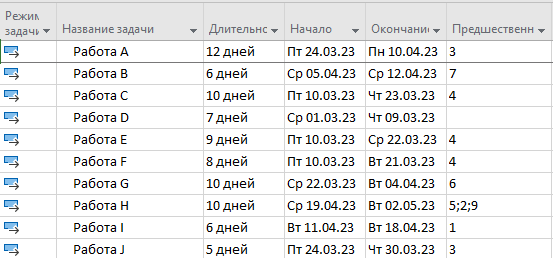
\includegraphics[scale=1.0]{imgs/task_0_0.png}
	\end{center}
	\caption{Решение тренировочного задания}
	\label{img:label}
\end{figure}

\begin{figure}[H]
	\begin{center}
		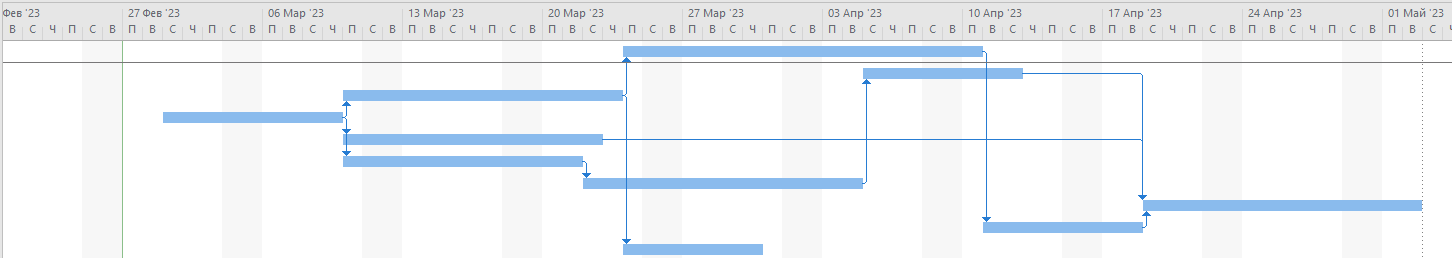
\includegraphics[width=\textwidth]{imgs/task_0_1.png}
	\end{center}
	\caption{Решение тренировочного задания (диаграмма Ганта)}
	\label{img:label}
\end{figure}